%\documentclass[mathserif]{beamer}
\documentclass[handout]{beamer}
%\usetheme{Goettingen}
\usetheme{Warsaw}
%\usetheme{Singapore}
%\usetheme{Frankfurt}
%\usetheme{Copenhagen}
%\usetheme{Szeged}
%\usetheme{Montpellier}
%\usetheme{CambridgeUS}
%\usecolortheme{}
%\setbeamercovered{transparent}
\usepackage[english, activeacute]{babel}
\usepackage[utf8]{inputenc}
\usepackage{amsmath, amssymb}
\usepackage{dsfont}
\usepackage{graphics}
\usepackage{cases}
\usepackage{graphicx}
\usepackage{pgf}
\usepackage{epsfig}
\usepackage{amssymb}
\usepackage{multirow}	
\usepackage{amstext}
\usepackage[ruled,vlined,lined]{algorithm2e}
\usepackage{amsmath}
\usepackage{epic}
\usepackage{epsfig}
\usepackage{fontenc}
\usepackage{framed,color}
\usepackage{palatino, url, multicol}
\usepackage{listings}
%\algsetup{indent=2em}
\newcommand{\factorial}{\ensuremath{\mbox{\sc Factorial}}}
\newcommand{\BIGOP}[1]{\mathop{\mathchoice%
{\raise-0.22em\hbox{\huge $#1$}}%
{\raise-0.05em\hbox{\L
\usepackage{fontenc}
\usepackage{framed,color}
\usepackage{palatino, url, multicol}
\usepackage{listings}
%\algsetup{indent=2em}
\newcommand{\factorial}{\ensuremath{\mbox{\sc Factorial}}}
\newcommand{\BIGOP}[1]{\mathop{\mathchoice%
{\raise-0.22em\hbox{\huge $#1$}}%
{\raise-0.05em\hbox{\Large $#1$}}{\hbox{\large $#1$}}{#1}}}
\newcommand{\bigtimes}{\BIGOP{\times}}
\vspace{-0.5cm}
\title{Introduction to Statistical Inference}
\vspace{-0.5cm}
\author[Felipe Bravo Márquez]{\footnotesize
%\author{\footnotesize  
 \textcolor[rgb]{0.00,0.00,1.00}{Felipe José Bravo Márquez}} 
\date{ \today }
arge $#1$}}{\hbox{\large $#1$}}{#1}}}
\newcommand{\bigtimes}{\BIGOP{\times}}
\vspace{-0.5cm}
\title{Introduction to Statistical Inference}
\vspace{-0.5cm}
\author[Felipe Bravo Márquez]{\footnotesize
%\author{\footnotesize  
 \textcolor[rgb]{0.00,0.00,1.00}{Felipe José Bravo Márquez}} 
\date{ \today }


\begin{document}
\begin{frame}
\titlepage


\end{frame}


%%%%%%%%%%%%%%%%%%%%%%%%%%%

% Useful references: http://www.buders.com/UNIVERSITE/Universite_Dersleri/istatistik/sampling_distributions_and_point_estimation_of_parameters.pdf
% http://homepage.divms.uiowa.edu/~rdecook/stat2020/notes/ch7_pt1.pdf

\begin{frame}{Populations and Samples}
\scriptsize{
\begin{itemize}
 \item The main goal of statistical inference is investigate properties about a target \textbf{population}.
 \item Example: What is the average height of the Chilean people? 
  \item In order to draw conclusions about a \textbf{population}, it is generally not feasible to gather all the data about it.
 \item We must make reasonable conclusions about a population based on the evidence provided by \textbf{sample data}.

 \item A \textbf{sample staticic} or simply \textbf{statistic} is a quantitative measure calculated from the data. Examples: the mean, the standard deviation, the minimum, the maximum.
 
 
 \item Our goal in sampling is to determine the value of a statistic for an entire population of interest, using just a small subset of the population.
 
 \item We do this primarily to save time and effort.
 
 \item Idea: Why go to the trouble of measuring every individual in the population when just a small sample is sufficient to accurately estimate the statistic of interest? \cite{poldrack2019statistical}
 
 

\end{itemize}

} 
\end{frame}


\begin{frame}{Statistical Inference (2)}
\scriptsize{
\begin{itemize}
 \item The process of drawing conclusions about a population from sample data is known as \textbf{statistical inference}.
\item In statistical inference we try to \textbf{infer} the distribution that generates the observed data.
\item Example: Given a sample $X_1, \dots, X_n \sim F$, how do we infer $F$? 
\item However, in most cases we are only interested in inferring some property of $F$ (e.g., its \textbf{mean} value).
\item Statistical models that assume that the distribution can be modeled with a finite set of parameters $\theta= (\theta_{1},\theta_{2},\dots,\theta_{k})$ are called \textbf{parametric models}. 
\item Example: if we assume that the data comes from a normal distribution $N(\mu,\sigma^2)$, $\mu$ and $\sigma$ would be the parameters of the model. 
\end{itemize}

} 
\end{frame}


\begin{frame}{Frequentist Aproaches}
\scriptsize{
The satistical methods to be presented is this class are known as \textbf{frequentist (or classical)} methods. They are based on the following postulates  \cite{wasserman2013all}:
\begin{itemize}
\item Probability refers to limiting relative frequencies. Probabilities are objective properties of the real world.
\item Parameters are fixed, unknown constants. Because they are not fluctuating, no useful probability statements can be made about parameters.
\item Statistical procedures should be designed to have well-defined long run frequency properties. For example, a 95 percent confidence interval should trap the true value of the parameter with limiting frequency at least 95 percent.
\end{itemize}
There is another approach to inference called \textbf{Bayesian inference}, which is based on different posulated, to be discussed later in the course.

} 
\end{frame}

\section{Point Estimation}

\begin{frame}{Point Estimation}
\scriptsize{
\begin{itemize}
 \item Point estimation is the process of finding the \textbf{best guess} for some quantity of interest from a \textbf{statistical sample}.
 \item In a general sence, this quantity of interest could be a parameter in a parametric model, a CDF $F$, a probability density function $f$, a regression function $r$, or a prediction for a future value $Y$ of some random variable.
 \item In this class we will consider this quantity of interest as a \textbf{population parameter} $\theta$. 
  \item By convention, we denote a point estimate of $\theta$ by $\hat{\theta}$ or $\hat{\theta}_n$.
 \item It is important to remark that while $\theta$ is an unknown fixed value, $\hat{\theta}$  depends on the data and is therefore a random variable. 
 \item We need to bear in mind that the process of sampling is by definition a random experiment. 
 
\end{itemize}

} 
\end{frame}

\begin{frame}{Point Estimation}

%http://homepage.divms.uiowa.edu/~rdecook/stat2020/notes/ch7_pt1.pdf

\scriptsize{
\begin{block}{Formal Definition}
\begin{itemize}
 \item Let $X_1, \dots, X_n$ be $n$ IID data points  from some distribution  $F$.
 \item A point estimator $\hat{\theta}_n$  of a parameter $\theta$ is some function of $X_1, \dots, X_n$:
 \begin{displaymath}
 \hat{\theta}_n=g(X_1, \dots, X_n) 
 \end{displaymath}
 
\end{itemize}

 
\end{block}

\begin{itemize}
 \item The \textbf{bias} of an estimator is defined as: 
\begin{displaymath}
 \text{bias}(\hat{\theta}_n)=\mathbb{E}(\hat{\theta}_n)-\theta
\end{displaymath}
\item An estimator is unbiased if $\mathbb{E}(\hat{\theta}_n)=\theta$ or  $\text{bias}(\hat{\theta}_n)=0 $
\end{itemize}

} 
\end{frame}


\begin{frame}{Sample Distribution}

\scriptsize{

\begin{itemize}
\item If we take multiple samples, the value of our statistical estimate $\hat{\theta}_n$ will also vary from sample to sample.

\item We refer to this distribution of our estimator across samples as the   \textbf{sampling distribution} \cite{poldrack2019statistical}.

\item The sampling distribution may be considered as the distribution of  $\hat{\theta}_n$ for all possible samples from the same population of size $n$\footnote{\url{https://courses.lumenlearning.com/boundless-statistics/chapter/sampling-distributions/}}.

\item We need to bear in mind this is an imaginary concept, since we can't obtain all possible samples.

\end{itemize}

} 
\end{frame}


\begin{frame}{Standard Error}

\scriptsize{

\begin{itemize}
\item The standard deviation of $\hat{\theta}_n$ is called the \textbf{standard error} $se$:
\begin{displaymath}
se(\hat{\theta}_n)=\sqrt{\mathbb{V}(\hat{\theta}_n})
\end{displaymath}
\item The standard error tells us about the variability of the estimator between all possible samples of the same size.
\end{itemize}

} 
\end{frame}





\begin{frame}{The Sample Mean}
\scriptsize{

\begin{itemize}
 \item Let $X_1,X_2,\dots,X_n$ be a random sample of a population of mean $\mu$ and variance $\sigma^2$
 \item  A sample statistic we can derive from the data is the  \textbf{sample mean} $\overline{X_{n}}$
 \begin{displaymath}
  \overline{X_{n}}=\frac{1}{n}\sum_{i=1}^{n} X_i
 \end{displaymath}
 \item The sample mean is a statitical estimate of the mean $\overline{X_{n}} = \hat{\mu}$.
 \item The sampling distribution of the sample mean: 
 
 
\item We can show that the sample mean is an unbiased estimator of $\mu$:
\begin{displaymath}
\mathbb{E}(\overline{X_{n}}) = \mathbb{E}(\frac 1n \sum_{i=1}^{n} X_i)  =  \frac 1n \times \mathbb{E}(\sum_{i=1}^{n} X_i) = \frac 1n (n \times \mu) = \mu  
\end{displaymath}
\end{itemize}

} 
\end{frame}

\begin{frame}{Point Estimation (4)}
\scriptsize{

\begin{itemize}
\item The standard error of the sample mean $se(\overline{X_{n}}) = \sqrt{\mathbb{V}(\overline{X_{n}})}$ can be calulated as:
\begin{displaymath}
 \mathbb{V}(\overline{X_{n}})=\mathbb{V}(\frac 1n \sum_{i=1}^{n} X_i) = \frac{1}{n^2} \mathbb{V}(\sum_{i=1}^{n} X_i) = \frac{n}{n^2} \mathbb{V}(X_i)=\frac{\sigma^2}{n} 
\end{displaymath}

\item Then,  $se(\overline{X_{n}}) = \frac{\sigma}{\sqrt{n}}$

\end{itemize}


} 
\end{frame}



\begin{frame}{Ejemplos de Estimación Puntual (5)}
\scriptsize{
\begin{itemize}
 \item Por lo general no sabemos $\sigma$ de la población.
 \item Cuando queremos estimar la varianza de una población a partir de una muestra hablamos de la  \textbf{varianza muestral}:
\item Existen dos estimadores comunes, una versión sesgada \begin{displaymath}
 s_{n}^{2}= \frac{1}{n} \sum_{i}^{n}(X_{i}-\overline{X_{n}})^2
\end{displaymath}

\item Una versión sin sesgo \begin{displaymath}
 s^{2}= \frac{1}{n-1} \sum_{i}^{n}(X_{i}-\overline{X_{n}})^2
\end{displaymath}

\item Cuando no sabemos la varianza de la población y queremos estimar la media, el error estándar es estimado: \begin{displaymath}                                                                                                                 
\hat{se}(\overline{X_{n}}) = \frac{s}{\sqrt{n}}                                                                                                                \end{displaymath}


\end{itemize}


} 
\end{frame}


\begin{frame}{Estimación Puntual (6)}
\scriptsize{
\begin{itemize}
 \item Sean $X_1, \dots, X_n \sim$ Bernoulli$(p)$ y sea $\hat{p}_{n}=\frac 1n \sum_{i}X_{i}$
 \item Luego $\mathbb{E}(\hat{p}_{n})= \frac 1n \sum_i \mathbb{E}(X_i)=p$, entonces $\hat{p}_n$ es insesgado.
 \item El error estándar $se$ sería
\begin{displaymath}
se = \sqrt{\mathbb{V}(\hat{p}_n)}= \sqrt{p(1-p)/n} 
\end{displaymath}
\item El error estándar estimado $\hat{se}$:
\begin{displaymath}
\hat{se} =\sqrt{\hat{p}(1-\hat p)/n} 
\end{displaymath}

\end{itemize}


} 
\end{frame}




\begin{frame}{Estimación Puntual (7)}

\scriptsize{

\begin{itemize}
\item Se espera que un buen estimador sea insesgado y de mínima varianza.

\item Unbiased ness used to receive much attention but these days is considered less important

\item Many of the estimators we will use are biased. 

\item A reasonable requirement for an estimator is that it should converge to the true parameter value as we collect more and more data.

\item Un estimador puntual $\hat{\theta}_n$ de un parámetro $\theta$ es \textbf{consistente} si converge al valor verdadero cuando el número de datos de la muestra tiende a infinito.
\item La calidad de un estimador se puede medir usando el \textbf{error cuadrático medio} (MSE)
\begin{displaymath}
MSE = \mathbb{E}_{\theta}(\hat{\theta}_n - \theta)^2 
\end{displaymath}

\end{itemize}

} 
\end{frame}



\begin{frame}{Estimación Puntual (8)}

\scriptsize{

\begin{itemize}
\item Si para un estimador $\hat{\theta}_n$, su $bias \rightarrow 0$ y su $se \rightarrow 0$ cuando $n\rightarrow \infty$, $\hat{\theta}_n$ es un estimador consistente de $\theta$.

\item Por ejemplo, para la media muestral $\mathbb{E}(\overline{X_{n}})=\mu$ lo que implica que el $bias =0$ y $se(\overline{X_{n}}) = \frac{\sigma}{\sqrt{n}}$ que tiende a cero cuando $n\rightarrow \infty$. Entonces $\overline{X_{n}}$ es un estimador consistente de la media.  

\item Para el caso del experimento Bernoulli se tiene que $\mathbb{E}(\hat{p})=p \Rightarrow bias=0$ y $se = \sqrt{p(1-p)/n} \rightarrow 0$ cuando $n\rightarrow \infty$. Entonces $\hat{p}$ es un estimador consistente de $p$.


\end{itemize}

} 
\end{frame}



\begin{frame}{Intervalo de Confianza}
\scriptsize{
\begin{itemize}
 \item Sabemos que el valor de un estimador puntual \textbf{varía} entre una muestra y otra
 \item Es más razonable encontrar un \textbf{intervalo} donde sepamos que valor \textbf{real del parámetro} se encuentra dentro del intervalo con una cierta \textbf{probabilidad}.
 \item La forma general de un intervalo de confianza en las siguiente:
  \begin{displaymath}
   \text{Intervalo de Confianza} = \text{Estadístico Muestral} \ \pm \ \text{Margen de Error}
  \end{displaymath}
 \item Entre más ancho el intervalo mayor incertidumbre existe sobre el valor del parámetro.
\end{itemize}


}
 
\end{frame}


\begin{frame}{Intervalo de Confianza (2)}
\scriptsize{

\begin{block}{Definición}
\begin{itemize}
 \item Un \textbf{intervalo de confianza} para un parámetro poblacional desconocido $\theta$ con un \textbf{nivel de confianza} $1-\alpha$, es un intervalo $C_n = (a,b)$ donde:
\begin{displaymath}
 \mathbb{P}(\theta \in C_n) = 1-\alpha
\end{displaymath}
 \item Además $a= a(X_1, \dots, X_n)$ y $b=b(X_1,\dots,X_n)$ son funciones de los datos
 \item El valor $\alpha$ se conoce como el nivel de \textbf{significancia}, generalmente se toma como $0.05$ lo que equivale a trabajar con un nivel de confianza de $95\%$
 \item La significancia se puede interpretar como la probabilidad de equivocarnos.
\end{itemize}

\end{block}

}
 
\end{frame}


\begin{frame}{Intervalo de Confianza (3)}
\scriptsize{

\begin{block}{Interpretación}
\begin{itemize}
 \item Existe mucha \textbf{confusión} de como interpretar un intervalo de confianza
 \item Una forma de interpretarlos es decir que si repetimos \textbf{un mismo experimento} muchas veces, el intervalo contendrá el valor del parámetro el $(1-\alpha)\%$ de las veces.
 \item Esta interpretación es correcta, pero rara vez repetimos un mismo experimento varias veces.
 \item Una interpretación mejor: un día recolecto datos creo un intervalo de $95\%$ de confianza para un parámetro $\theta_1$. Luego, en el día 2 hago lo mismo para un parámetro $\theta_2$ y así reiteradamente $n$ veces. El $95\%$ de mis intervalos \textbf{contendrá} los valores reales de los parámetros.
 
\end{itemize}

\end{block}

}
 
\end{frame}

\begin{frame}{Intervalo de Confianza (4)}
\scriptsize{
\begin{itemize}
 \item Se tienen $n$ observaciones independientes $X_1, \dots, X_n$ IID de distribución  $N(\mu,\sigma^2)$
 \item Supongamos que $\mu$ es \textbf{desconocido} pero $\sigma^2$ es \textbf{conocido}.
 \item Sabemos que $\overline{X_{n}}$ es un estimador insesgado de $\mu$
 \item Por la ley de los grandes números sabemos que la distribución de $\overline{X_{n}}$ se concentra alrededor de $\mu$ cuando $n$ es grande.
 \item Por el CLT sabemos que \begin{displaymath}
 Z=\frac{\overline{X_{n}}-\mu}{\frac{\sigma}{\sqrt{n}}}  \sim N(0,1)
\end{displaymath}
cuando $n$ es grande
\item Despejando, tenemos que $\mu = \overline{X_{n}} - \frac{\sigma}{\sqrt{n}}Z$
\end{itemize}


 }
\end{frame}

\begin{frame}{Intervalo de Confianza (5)}
\scriptsize{
\begin{itemize}
 \item Queremos encontrar un intervalo intervalo $C_n = (\mu_1,\mu_2)$ con un nivel de confianza $1-\alpha$:
\begin{displaymath}
 \mathbb{P}(\mu_1 \leq \mu \leq \mu_2 ) = 1-\alpha
\end{displaymath}
\item Sea $z_a = \Phi^{-1}(1-a)$, con $a \in [0,1]$ donde $\Phi^{-1}$ es la función cuantía de una normal estandarizada
\item Esto es equivalente a decir que $z_a$ es el valor tal que $1-\Phi(z_a)=\mathbb{P}(Z \geq z_a)=a$

\item Por simetría de la normal $z_{\alpha/2}=-z_{(1-\alpha/2)}$
\end{itemize}


 }
\end{frame}



\begin{frame}{Intervalo de Confianza (6)}
\scriptsize{
\begin{itemize}
 \item Se tiene que \begin{displaymath}
\mathbb{P}(-z_{\alpha/2}<Z<z_{\alpha/2})=1-\alpha                     
                    \end{displaymath}

\begin{figure}[h!]
	\centering
	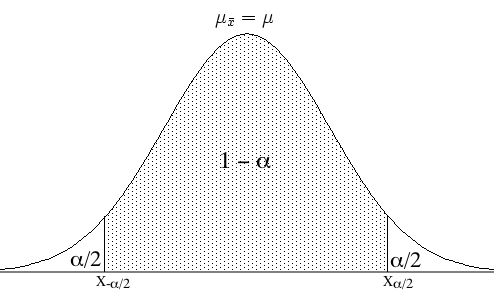
\includegraphics[scale=0.35]{pics/ConfIntervNormalP.png}
\end{figure}




\end{itemize}
}
 
\end{frame}

\begin{frame}{Intervalo de Confianza (7)}
\scriptsize{
\begin{itemize}
 \item  El intervalo de confianza para $\mu$ es:
 \begin{displaymath}
 C_n = (\overline{X_{n}}-z_{\alpha/2}\frac{\sigma}{\sqrt{n}} , \overline{X_{n}} + z_{\alpha/2}\frac{\sigma}{\sqrt{n}}) 
 \end{displaymath}
\item Entonces $ z_{\alpha/2}$ nos dice cuantas veces tenemos que multiplicar el \textbf{error estándar} en el intervalo.
\item Mientras menor sea $\alpha$ mayor será $ z_{\alpha/2}$ y por ende más ancho será el intervalo. 
\item Demostración:
 \begin{eqnarray*}
 \mathbb{P}(\mu \in C_n) & = & \mathbb{P}(\overline{X_{n}}-z_{\alpha/2}\frac{\sigma}{\sqrt{n}} < \mu < \overline{X_{n}} + z_{\alpha/2}\frac{\sigma}{\sqrt{n}}) \nonumber \\ 
                         & = & \mathbb{P}(-z_{\alpha/2} < \frac{\overline{X_{n}}-\mu}{\frac{\sigma}{\sqrt{n}}} <  z_{\alpha/2}) \nonumber \\ 
			  & = & \mathbb{P}(-z_{\alpha/2} < Z <  z_{\alpha/2}) \nonumber \\
			   & = & 1-\alpha 
 \end{eqnarray*}


\end{itemize}
}


 
\end{frame}

\begin{frame}[fragile]{Intervalo de Confianza (8) }

\scriptsize{
\begin{itemize}
 \item Como $z_{\alpha/2} = \Phi^{-1}(1-\alpha/2)$ podemos usar la función cuantía de la normal para calcular intervalos de confianza en R
\end{itemize}


\begin{verbatim}
> alpha <- 0.05
> xbar <- 5
> sigma <- 2
> n <- 20
> se <-sigma/sqrt(n)
> error <- qnorm(1-alpha/2)*se
> left <- xbar-error
> right <- xbar+error
> left
[1] 4.123477
> right
[1] 5.876523
>
\end{verbatim}
}



\end{frame}

\begin{frame}{Distribución T}
\scriptsize{
\begin{itemize}
 \item En la pŕactica, si no conocemos $\mu$ es poco probable que conozcamos $\sigma$
 \item Si estimamos $\sigma$ usando $s$, los intervalos de confianza se construyen usando la distribución \textbf{T-student}
\end{itemize}

\begin{block}{Distribución T}
\begin{itemize}
 \item Una V.A tiene distribución $t$ con $k$ grados de libertad cuando tiene la siguiente PDF:
\begin{displaymath}
 f(t)=\frac{\Gamma(\frac{k+1}{2})}{\sqrt{k\pi}\Gamma(\frac k2)(1+\frac{t^2}{k})^{(k+1)/2}}
\end{displaymath}
\item Cuando $k=1$ se le llama distribución de \textbf{Cauchy}
\item Cuando $k\rightarrow \infty$ converge a una distribución normal estandarizada
 \item La distribución t tiene colas más anchas que la normal cuando tiene pocos grados de libertad


\end{itemize}

 
\end{block}




} 
\end{frame}

\begin{frame}[fragile]{Distribución T (2)}
 \scriptsize{



\begin{verbatim*}
x<-seq(-8,8,length=400)
y1<-dnorm(x)
y2<-dt(x=x,df=1)
y3<-dt(x=x,df=10)
y4<-dt(x=x,df=350)
plot(y1~x,type="l",col="green")
lines(y2~x,type="l",col="blue")
lines(y3~x,type="l",col="black")
lines(y4~x,type="l",col="red")

\end{verbatim*}

 \begin{figure}[h!]
	\centering
	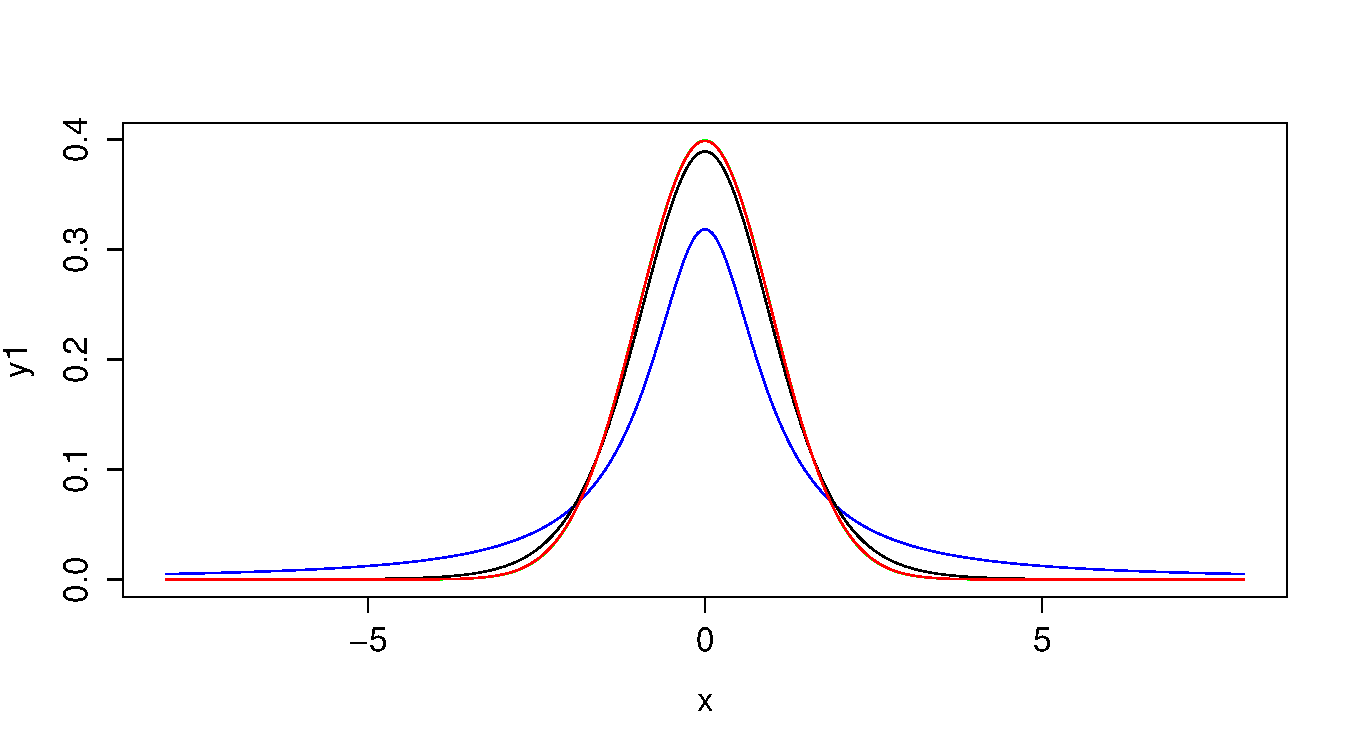
\includegraphics[scale=0.3]{pics/tstudent.pdf}
\end{figure}


}
\end{frame}


\begin{frame}{Intervalo de Confianza (9) }

\scriptsize{
\begin{itemize}
 \item Sea  $s^{2}= \frac{1}{n-1} \sum_{i}^{n}(X_{i}-\overline{X_{n}})^2$ tenemos:
 \begin{displaymath}
  T=\frac{\overline{X_{n}}-\mu}{\frac{s}{\sqrt{n}}}\sim t_{n-1}
 \end{displaymath}
\item Sea $t_{n-1,a}=\mathbb{P}(T>a)$, equivalente a la función cuantía $qt$ evaluada en $(1-a)$
\item El intervalo de confianza resultante es:
       \begin{displaymath}
 C_n = (\overline{X_{n}}-t_{n-1,\alpha/2}\frac{s}{\sqrt{n}} , \overline{X_{n}} + t_{n-1,\alpha/2}\frac{s}{\sqrt{n}}) 
 \end{displaymath} 
 \item Como las colas de la distribución $t$ son más anchos cuando $n$ es pequeño, los intervalos de confianza resultantes son más anchos

\end{itemize}


}

\end{frame}


\begin{frame}[fragile]{Intervalo de Confianza (10)}
\scriptsize{
\begin{itemize}
 \item Calculemos un intervalo de confianza para la media de \verb+Petal.Length+ de los datos del \textbf{Iris} con $95\%$ de confianza
\begin{verbatim}
>data(iris)
>alpha<-0.05
>n<-length(iris$Petal.Length)
>xbar<-mean(iris$Petal.Length)
>xbar
[1] 3.758
>s<-sd(iris$Petal.Length)
>se<-s/sqrt(n)
>error<-qt(p=1-alpha/2,df=n-1)*se
>left<-xbar-error
>left
[1] 3.473185
>right<-xbar+error
>right
[1] 4.042815
\end{verbatim}
\item Otra forma:
\begin{verbatim}
>test<-t.test(iris$Petal.Length,conf.level=0.95)
>test$conf.int
[1] 3.473185 4.042815
\end{verbatim}


\end{itemize}



}
 
\end{frame}

\begin{frame}{Test de Hipótesis}
\scriptsize{
\begin{itemize}
 \item Cuando queremos probar si alguna \textbf{propiedad} asumida sobre una población se contrasta con una muestra estadística usamos un \textbf{Test de Hipótesis}
\item El test se compone de las siguientes hipótesis:
 \begin{itemize}
\scriptsize{
\item \textbf{Hipótesis Nula} $H_{0}$: Simboliza la situación actual. Lo que se ha considerado real hasta el presente.
\item \textbf{Hipótesis Alternativa} $H_{a}$: es el modelo alternativo que queremos considerar. 
}
 \end{itemize}
\item La idea es encontrar suficiente \textbf{evidencia estadística} para rechazar $H_{0}$ y poder concluir $H_{a}$
\item Si no tenemos suficiente evidencia estadística \textbf{fallamos en rechazar} $H_{0}$

\end{itemize}



} 
\end{frame}



\begin{frame}{Test de Hipótesis (2)}
\scriptsize{

\begin{block}{Metodología para Realizar un Test de Hipótesis}
\begin{itemize}
 \item Elegir una hipótesis nula $H_0$ y alternativa $H_a$
 \item Fijar un nivel de significancia $\alpha$ del test
 \item Calcular un estadístico $T$ a partir de los datos
 \item El estadístico $T$ es generalmente un valor estandarizado que podemos chequear en una tabla de distribución
 \item Definir un criterio de rechazo para la hipótesis nula. Generalmente es un valor crítico $c$.
\end{itemize}
\end{block}



} 
\end{frame}



\begin{frame}[fragile]{Test de Hipótesis (3)}
\scriptsize{
\begin{itemize}
 \item Ejemplo: Se sabe que la cantidad de horas promedio de uso de Internet mensual en Chile país es de 30 horas
 \item Supongamos que queremos demostrar que el promedio es distinto a ese valor.
 \item Tendríamos que $H_0: \mu=30$ y $H_{a}: \mu \neq 30$
 \item Fijamos $\alpha=0.05$ y recolectamos 100 observaciones
 \item Supongamos que obtenemos $\overline{X_{n}}=28$ y $s=10$
 \item Una forma de hacer el test es construir un intervalo de confianza para $\mu$ y ver si $H_{0}$ está en el intervalo.
\begin{verbatim}
> 28-qt(p=0.975,99)*10/sqrt(100)
[1] 26.01578
> 28+qt(p=0.975,99)*10/sqrt(100)
[1] 29.98422 
\end{verbatim}
\item El intervalo sería la zona de aceptación de $H_0$ y todo lo que esté fuera de éste será mi región de rechazo.
\item Como 30 está en la región de rechazo, rechazo mi hipótesis nula con un $5\%$ de confianza.
\end{itemize}



} 
\end{frame}


\begin{frame}[fragile]{Test de Hipótesis (4)}
\scriptsize{
\begin{itemize}
 \item Otra forma de realizar el test es calcular el estadístico $T=\frac{\overline{X_{n}}-\mu_{o}}{\frac{s}{\sqrt{n}}}$
 \item En este caso sería \begin{displaymath}
                           T=\frac{28-30}{\frac{10}{\sqrt{100}}}=-2
                          \end{displaymath}
\item Como $H_{a}: \mu \neq 30$, tenemos un test de dos lados, donde la región de aceptación es
\begin{displaymath}
 t_{n-1,1-\alpha/2}<T<t_{n-1,\alpha/2}
\end{displaymath}
\begin{verbatim}
 > qt(0.025,99)
[1] -1.984217
> qt(0.975,99)
[1] 1.984217
\end{verbatim}
\item Como $T$ está en la región de rechazo, rechazamos la hipótesis nula.

\end{itemize}



} 
\end{frame}


\begin{frame}[fragile]{Test de Hipótesis (5)}
\scriptsize{
\begin{itemize}
 \item Generalmente, además de saber si rechazamos o fallamos en rechazar una hipótesis nula queremos saber la evidencia que tenemos en contra de ella.
 \item Se define un \textbf{p-valor} como la probabilidad de obtener un resultado al menos tan extremo como el observado en los datos dado que la hipótesis nula es verdadera.
 \item ``Extremo'' significa lejos de la hipótesis nula.
 \item Si el \textbf{p-valor} es menor que el nivel de significancia $\alpha$, rechazamos $H_{0}$ 
 \item Ejemplo:
\begin{verbatim}
> data(iris)
> mu<-3 # La hipótesis nula
> alpha<-0.05
> n<-length(iris$Petal.Length)
> xbar<-mean(iris$Petal.Length)
> s<-sd(iris$Petal.Length)
> se<-s/sqrt(n)
> t<-(xbar-mu)/(s/sqrt(n))
> pvalue<-2*pt(-abs(t),df=n-1)
> pvalue
[1] 4.94568e-07 # es menor que 0.05 entonces rechazamos H0
\end{verbatim}
\end{itemize}

 


}
\end{frame}

\begin{frame}[fragile]{Test de Hipótesis (6)}
\scriptsize{
\begin{itemize}
 \item La forma elegante de hacerlo en R:
\end{itemize}

\begin{verbatim}
> t.test(x=iris$Petal.Length,mu=3)

	One Sample t-test

data:  iris$Petal.Length 
t = 5.2589, df = 149, p-value = 4.946e-07
alternative hypothesis: true mean is not equal to 3 
95 percent confidence interval:
 3.473185 4.042815 
sample estimates:
mean of x 
    3.758 
\end{verbatim}
}



\end{frame}

\begin{frame}{Test de Hipótesis (7)}
 \scriptsize{

\begin{itemize}
 \item Tenemos dos tipos de errores cuando realizamos un test de hipótesis
 \item Error tipo I: es cuando rechazamos la hipótesis nula cuando ésta es cierta.
 \item Este error es equivalente al nivel de significancia $\alpha$
 \item Error tipo II: es cuando la hipótesis nula es falsa pero no tenemos evidencia estadística para rechazarla.
 \item Para mitigar los errores tipo I generalmente usamos valores de $\alpha$ más pequeños.
 \item Para mitigar los errores tipo II generalmente trabajamos con muestras más grandes.
 \item Existe un trade-off entre los errores tipo I y tipo II. 
\end{itemize}

 \begin{table}
\begin{tabular}{c | c c}
\hline
  & Retener $H_0$ &  Rechazar $H_{0}$   \\ 
\hline
$H_0$ es verdadera & \checkmark & error tipo I \\
$H_1$ es verdadera & error tipo II & \checkmark \\
\hline
\end{tabular}
\end{table}

}
\end{frame}

\begin{frame}{Statistical Power}
 
\end{frame}

\begin{frame}{Critics to Hypothesis Testing}
 
\end{frame}

\begin{frame}{Maximum Likelihood Estimation}
 
\end{frame}


%%%%%%%%%%%%%%%%%%%%%%%%%%%
%%%%%%%%%%%%%%%%%%%%%%%%%%%
\begin{frame}[allowframebreaks]\scriptsize
\frametitle{References}
\bibliography{bio}
\bibliographystyle{apalike}
%\bibliographystyle{flexbib}
\end{frame}  









%%%%%%%%%%%%%%%%%%%%%%%%%%%

\end{document}
